\documentclass{standalone}

\usepackage{tikz}
\usetikzlibrary{backgrounds, positioning, decorations.pathreplacing, calc, fit}
\usetikzlibrary{shapes}

\begin{document}

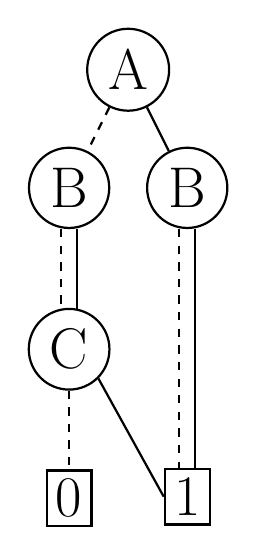
\begin{tikzpicture}
    \tikzstyle{inner} = [draw, solid, circle, thick];
    \tikzstyle{terminal} = [draw, solid, rectangle, thick];

    \node[inner] at (0, 0) (A) {\huge{A}}
    child[thick, dashed] { node[inner] (Bl) {\huge{B}} }
    child[thick] { node[inner] (Br) {\huge{B}} };

    \node[inner, below = 1 of Bl] (C) {\huge{C}};
    \node[terminal, below = 3.0325 of Br] (1) {\huge{1}};
    \node[terminal, below = 1 of C] (0) {\huge{0}};

    \draw[thick, dashed] (Bl.south) ++(-0.1, 0) -- ++(0, -1.025);
    \draw[thick] (Bl.south) ++(0.1, 0) -- ++(0, -1.025);

    \draw[thick, dashed] (Br.south) ++(-0.1, 0) -- ++(0, -3.0325);
    \draw[thick] (Br.south) ++(0.1, 0) -- ++(0, -3.0325);

    \draw[thick, dashed] (C.south) -- (0.north);
    \draw[thick] (C.south east) -- (1.west);
\end{tikzpicture}

\end{document}